% Created 2012-06-17 Sun 13:00
\documentclass{article}
\usepackage[utf8]{inputenc}
\usepackage[T1]{fontenc}
\usepackage{fixltx2e}
\usepackage{graphicx}
\usepackage{longtable}
\usepackage{float}
\usepackage{wrapfig}
\usepackage{soul}
\usepackage{textcomp}
\usepackage{marvosym}
\usepackage{wasysym}
\usepackage{latexsym}
\usepackage{amssymb}
\usepackage{hyperref}
\tolerance=1000
\usepackage{mathrsfs}
\usepackage{graphicx}
\usepackage{hyperref}
\usepackage{subfigure}
\usepackage[textwidth=16cm,textheight=24cm]{geometry}
\providecommand{\alert}[1]{\textbf{#1}}

\title{Simulation in Industrial Organization}
\author{Dan Hammer}
\date{\today}
\hypersetup{
  pdfkeywords={},
  pdfsubject={},
  pdfcreator={Emacs Org-mode version 7.8.02}}

\begin{document}

\maketitle

\newcommand{\sss}{$s^2$ }
\newcommand{\R}{\texttt{R} }
\newcommand{\ep}{{\bf e}^\prime}
\newcommand{\e}{{\bf e}}
\newcommand{\Rs}{R^2}
\newcommand{\yp}{{\bf y}^\prime}
\newcommand{\y}{{\bf y}}
\newcommand{\X}{{\bf X}}
\newcommand{\Q}{{\bf Q}}
\newcommand{\J}{{\bf J}}
\newcommand{\Xp}{{\bf X}^{\prime}}
\newcommand{\Z}{{\bf Z}}
\newcommand{\Zp}{{\bf Z}^{\prime}}
\renewcommand{\P}{{\bf P}}
\renewcommand{\Pp}{{\bf P}^{\prime}}
\renewcommand{\In}{{\bf I}_n}
\newcommand{\Zin}{(\Zp\Z)^{-1}}
\newcommand{\E}{\mathbb{E}}
\newcommand{\V}{\mathbb{V}}
\newcommand{\sigs}{\sigma^2}


I have just taken a graduate-level course in industrial organization.  It has become clear that the heuristic models that are used to teach the core concepts are somewhat fragile.  In some cases, relaxing assumptions only slightly yields a very different set of conclustions -- some of which are counterintuitive.  The purpose of the models -- as I understand it -- is to provide some structure to empirical study; to offer a testable hypothesis based on economic insight.  The problem, here, is that by relaxing the (ver strict) assumptions, the conclusions are often subject to massive swings in both implied magnitude and directionality of the model impacts.  The following set of examples illustrate that just about any outcome is feasible -- even within the constraints of the model -- when just a little uncertainty is added to a few basic models.  

All of the supporting code is included in the public Github repository \href{https://github.com/danhammer/stat-computing}{\texttt{stat-computing}}, including the \texttt{org-mode} files that compile to this document.  Most of the examples can be found in the \href{https://github.com/danhammer/stat-computing/blob/master/src/computing/io-simulation.clj}{\texttt{io-simulation}} namespace.  The project is mainly written in Clojure; but a few examples are written in \texttt{R}.  Still, the project is structured as a Clojure project, with instructions on how to compile and run the examples in the front-page readme.

\section*{Existence of informed consumers}
\label{sec-1}


Consider a standard model of vertical product differentiation with $N$ consumers.  Of the $N$ consumers only a fraction $\alpha$ are informed; the rest are unable to distinguish between two quality levels $s=0$ and $s=1$ before the product is purchased.  Only one unit can be bought in this simple model.  Consumer preferences are identical for all consumers, with their utility function defined as follows:
\begin{equation}
U(\theta, s, p) = \left\{
  \begin{array}{ll}
        \theta s - p  & \mbox{if one unit is bought};\\
        0 & \mbox{otherwise}.
  \end{array} \right.
\end{equation}
where $p$ is the price of one unit of the product and $\theta$ is a parameter that represents the consumer's valuation of quality.  Suppose that the high quality product ($s=1$) is more expensive to produce, so that the marginal cost $c_1 > c_0$.  Assume that each firm in the competitive market can only produce one type of product.   Moreover, suppose that the uninformed consumer believes that high price signals high quality, whereas the informed consumer is able to infer quality by prior knowledge.  In this straightforward and abstracted model, the equilibrium price and quality are easily calculated.  

The informed consumers purchase the product if $s = 1$ and $p < \theta$.  The uninformed consumers always buy if the price is high.  The firm will choose $p$ and $s$ to maximize profits.  For any level of $s$, the profit-maximizing firm will always choose a high price, $p \equiv p^h$.  The firm's profits vary by quality level:
\[
\begin{array}{ll}
  s = 1: & \pi_1 = p - c_1 \\
  s = 0: & \pi_0 = (1 - \alpha)(p - c_0)
\end{array}
\]
The firm will choose to supply a high-quality product when $\pi_1 > \pi_0$, or equivalently when $p- c_1 > (1 - \alpha)(p - c_0)$.  Rearranging, the condition to supply a high-quality product is 
\begin{equation}
\label{e:high}
p > \frac{c_1 - (1-\alpha)c_0}{\alpha} = \frac{c_1 - c_0}{\alpha} + c_0
\end{equation}
It is clear from Equation (\ref{e:high}) that as the proportion of informed consumers increases (as $\alpha$ increases) the firms are more likely to supply a high-quality product; the right-hand side of the inequality becomes \emph{easier} to satisfy.  This makes sense.  With more informed consumers in the market, the firms are forced to supply a higher quality product to \emph{all} consumers.  The informed consumers impose a welcome, positive externality on the uninformed.

It is reasonable to assume that the true proportion of informed consumers in the market is not known to the firms.  Instead each firm has a perception of the true $\alpha$ and will make supply decisions accordingly.  The quality level is no longer consant across firms; each firm has an individual notion of the true proportion.  Suppose that these perceptions are normally distributed around the true proportion.  A natural question, then, is how the average quality changes as the spread around the true proportion increases.

Consider a dummy example where $c_0 = 2$; $c_1 = 5$; $p = 16$; and the true proportion $\alpha = 0.4$.  If $\alpha$ were known to all firms, then the right-hand side of Equation (\ref{e:high}) would be equal to 15.5, so that the inequality condition is \emph{always} satisfied.  The average product quality in the market would therefore be 1.  We can examine the effect of increased uncertainty about the true $\alpha$ by simulating a market with 10,000 firms.  Let $\hat{\alpha} \sim N(\alpha, \sigma^2)$ be the perceived proportion of informed buyers for each firm.  In this example, firm $i$ will choose to produce high quality goods if the following condition is met:
\begin{equation}
\label{e:est}
p > \frac{c_1 - c_0}{\hat{\alpha}_i} + c_0 \Rightarrow \hat{\alpha}_i > \frac{3}{14}
\end{equation}
We can therefore find the average quality as a function of $\sigma^2$ through Monte Carlo simulation, which will specify the effect of increased uncertainty on product quality in the market.  The code for this example is provided in the Github repository in the \texttt{io-simulation} namespace.  

The resulting graph is presented in Figure (\ref{f:mc}).  The variation around the curve is a result of the finite number of firms.  As the number of firms increases, the simulated results will be a tighter fit around the curve.  This example reflects the rate at which the area to the left of $3/14 \approx 0.214$ under a normal distribution with mean $0.4$ changes as the variance increases.

\begin{figure}[htb]
\centering
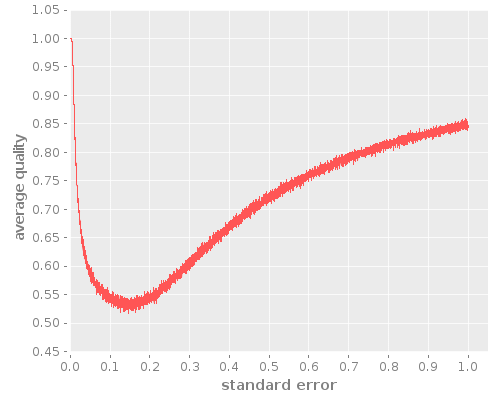
\includegraphics[width=10cm]{mc-est.png}
\caption{\label{f:mc}Average quality as a function of $\V(\hat{\alpha})$}
\end{figure}

The graph illustrates a common theme throughout this set of examples.  Introducing a small amount of uncertainty in a single parameter can change the interpretation of model parameters or even alter the implied direction of a model effect.  The shape of the function in Figure (\ref{f:mc}) may be interesting because it implies that, although the true proportion of informed consumers does not change, the uncertainty around that parameter has a non-monotonic effect on average product quality.  That is, over a certain range of uncertainty, firms will on average supply lower quality products.  As the uncertainty increases beyond a standard error of approximately 0.15, however, the effect is reversed: more uncertainty implies a higher average product quality.  

This example alone does not completely illustrate my overall point that model implications are very fragile and suceptible to change when subjected to slight uncertainty; but it does suggest that many outcomes may be feasible within the model's framework, depending on uncertainty and interactions between uncertain parameters.  In this case, the analysis does suggest a potentially testable hypothesis, but even this slightly more general hypothesis is fragile subject to uncertainty in other parameters.

\end{document}
